\chapter{Physics Practicals}

\section{Introduction to Physics Practicals}

\subsection{Format}
The format of the Physics practical exam was revised in 2011 to keep up with the 2007 updated syllabus. As such, there will be no further Alternative to Practical exams, pending approval from the Ministry of Education.

The Physics practical has 2 questions and students must answer both. Question 1 comes from Mechanics, and Question 2 can come from Heat, Light, Waves or Electricity. Each question is worth 25 marks, and students have 2$\frac{1}{2}$ hours to complete the exam.

\subsubsection{Physics 1 Theory Format}
The theory portion of the Physics exam comprises 100 marks, while the practical carries 50 marks. A student's final grade for Physics is thus found by taking her total marks from both exams out of 150.

The theory exam for Physics contains 3 sections. Section A has 3 questions and is worth 30 marks - Question 1 is 10 multiple choice, Question 2 is 10 matching, and Question 3 is 10 fill-in-the-blank. Section B has 6 long answer questions and is worth 60 marks. Section C has 2 questions regarding the use of apparatus and simple technological appliances in everyday life, though students must answer \textbf{only 1} of these questions. It is worth 10 marks.

\paragraph{Note} This information is current as of the time of publication of this manual. Updated information may be obtained by contacting the Ministry of Education. 

\subsection{Notes for Teachers}

\subsubsection{NECTA Advance Instructions}
Advance instructions are given to teachers at least one month before the date of the exam. However, unlike Biology and Chemistry, \textbf{there are no 24 hour advance instructions given for Physics}.

%[tips for identifying practicals from advance instructions, example advance instructions?]

\subsubsection{Words of Advice}
%Even for the experienced teacher, the physics practical can seem a daunting task.
%It has multiple sections spanning four years of a dense, unrelenting syllabus, combining
%physics and math topics alike that might or might not have been taught by previous
%teachers. Furthermore, the typical student in a secondary school will have little to no
%experience with common apparatus.

The Physics practical is different from the Chemistry and Biology practicals in that
the exams feature a greater variety of questions. That means we need to teach it all, even if the teacher before you never found his or her way into the classroom and you realize at the end of Form Four that the students still have not studied the Form Two syllabus. If you are teaching all forms, do not wait to start practicals until later forms; always do a practical when the corresponding topic comes up. In addition, train the students well in the general principles of collecting data, graphing data, and writing up experimental points. These skills are required in every physics practical, and carry most of the points.

The practical section of the exam is a third of a student’s total score, and fully half
of that is graphing and labeling experimental data. 
%There are typically three questions on
%the same general topics: mechanics, light and electricity. The students must answer the
%mechanics question, but they can choose between light and electricity. Most students tend
%to choose the light experiment as it is easier to understand and is generally taught more
%than the electricity topics. It is also easier to prepare as a teacher. However, this does not
%mean that the electricity practical is too difficult; if prepared well, it can actually be the
%easiest to perform provided the students have a clear understanding of the apparatus, and you have prepared and tested it well. This is where you come in.
Though the practical is varied, a student does not necessarily need a deep
understanding of the concept in question. If they are familiar with the apparatus and the
process of drawing and interpreting a graph, the practical should be quite simple.
Whenever possible, allow the students to play and experiment with the apparatus,
whether it is a metre bridge, mirror, pendulum, etc. If they have done each of these experiments several times, they will be confident in their ability.

The more familiar your students are with these techniques, the better they will do.
Perform these practicals as often as possible: when the topic comes up, when preparing
for the mock and NECTA exams, and any time you can get them to come in for an
evening session or a weekend. They will make many, many mistakes the first couple of
times through but that is exactly what you want as they will learn from their mistakes and
remember them.

%\subsection{NECTA Marking Information}
%[how NECTA marks the practicals, highlight most important parts]

\subsection{Common Practicals}
\begin{description} \itemsep1pt \parskip0pt \parsep0pt
\item[Mathematics]{a brief overview of some of the mathematical and graphing skills required to perform many of the common physics practicals}
\item[Mechanics] \hfill 
\begin{description} 
\item[Hooke's Law (Form 1)]{use a spring and various masses to determine either the spring constant or the value of an unknown mass graphically}
\item[Simple Pendulum (Form 2)]{find the acceleration due to gravity using a pendulum and stopwatch}
\item[Principle of Moments (Form 2)]{verify the Principle of Moments using masses and a ruler on a knife edge, or calculate the mass of a metre rule}
%\item[Archimedes' Principle (Form 1)]{verify Archimedes' Principle by measuring the volume of water displaced by an object submerged in a Eureka can}
\end{description}
\item[Light] \hfill 
\begin{description}
\item[Plane Mirror (Reflection) (Form 1)]{generally 3 varieties: find image distance, verify the Laws of Reflection, or find the number of images produced by two plane mirrors placed at different relative angles}
\item[Rectangular Prism (Refraction) (Form 3)]{find the refractive index or critical angle for a glass block by varying the angle of incidence and measuring the corresponding angles of refraction}
\end{description}
\item[Electricity] \hfill 
\begin{description} 
\item[Potentiometers]{find the drop in potential along a length of resistance wire}
\item[Metre Bridges]{determine the value of an unknown resistor using a known resistor and a galvanometer to find a point of equal potential along a resistance wire}
\item[Ohm's Law (Form 2)]{verify Ohm's Law or determine the internal resistance of a cell}
\end{description}
\end{description}

\paragraph{Note} These are the most common practicals, but they are not necessarily the only practicals that can occur on a NECTA exam. Physics practical questions can come from a variety of topics which may not yet have been used in older past papers. Be sure to regularly check the most recent \nameref{cha:past-papers-phys} to get a good idea of the types of questions to expect. 

\subsection{Recent Practicals}
Given below is an attempt to characterize the Physics practical questions from recent years according to category and topic. Each question is given with its corresponding topic on top and the objective, or what is to be solved for, on bottom. This information can be used to try and find trends in what exam writers like to test students on, and what topics are most likely to occur on an exam. However, nothing should be assumed to be a guarantee, and students should be well-prepared in all practicals so that they can take on any question they may face on the NECTA.

Note a few things from the table below:
\begin{itemize*}
\item Beginning in 2011, the format of the exam changed to consist of only 2 problems, one of which must come from Mechanics.
\item The exam committee has a tendency to repeat some problems. For example, the Mechanics questions from 2004 and 2011 are nearly identical, as are the Light questions from 2004 and 2008.
\end{itemize*}

\begin{center}
\begin{tabular}{|c|c|c|c|} \hline
\textbf{Year} & \textbf{Mechanics} & \textbf{Light} & \textbf{Electricity} \\ \hline
\multirow{2}{*}{2013} & Principle of Moments & Plane Mirror & \multirow{2}{*}{-----} \\
& \emph{verify} & \emph{object, image dist.} & \\ \hline
\multirow{2}{*}{2012} & Density & Plane Mirror & \multirow{2}{*}{-----} \\
& \emph{verify} $\rho = \frac{m}{V}$ & \emph{number of images} & \\ \hline
\multirow{2}{*}{2011} & Principle of Moments & \multirow{2}{*}{-----} & Ohm's Law \\
& \emph{mass of ``AA'' battery} & & \emph{e.m.f., int. resistance} \\ \hline
\multirow{2}{*}{2010} & Elasticity & Refraction & Ohm's Law \\
& \emph{unknown mass, $k$} & \emph{refr. index of water} & \emph{$\rho$ of a wire} \\ \hline
\multirow{2}{*}{2009} & Simple Pendulum & Refraction & Ohm's Law \\
& \emph{relate $l \rightarrow T$} & \emph{refr. index of glass} & \emph{verify $V = IR$} \\ \hline
\multirow{2}{*}{2008} & Elasticity & Refraction & Ohm's Law \\
& \emph{verify $F=kx$, find $k$} & \emph{$\cfrac{d\cos{r}}{\sin{(i-r)}}$}  & \emph{verify $V=IR$} \\ \hline
\multirow{2}{*}{2007} & Elasticity & Refraction & Potentiometer \\
& \emph{unknown mass, $k$} & \emph{refr. index of glass} & \emph{$\Delta V$ along wire} \\ \hline
\multirow{2}{*}{2006} & Elasticity & Plane Mirror & Metre Bridge \\
& \emph{unknown mass, $F = kx$} & \emph{object, image dist.} & \emph{unknown $R$} \\ \hline
\multirow{2}{*}{2005} & Elasticity & Refraction & Ohm's Law \\
& \emph{unknown mass, $k$} & \emph{critical angle} & \emph{e.m.f., int. resistance} \\ \hline
\multirow{2}{*}{2004} & Principle of Moments & Refraction & Potentiometer \\
& \emph{mass of ``AA'' battery} & \emph{$\cfrac{d\cos{r}}{\sin{(i-r)}}$} & \emph{$\rho$ of wire, int. res.} \\ \hline
\end{tabular}
\end{center}

%For a collection of NECTA past papers from the Physics Practical exam, see []

%==============================================================================

\section{Mathematics}

No physics experiment is complete without a healthy dose of graphing and
formulas. As math is typically the worst subject for most students, it is often upon the
physics teacher to drive home the understanding of how to draw and interpret graphs, as
well as how to apply formulas to those graphs. It comes down to a few simple things:
correctly setting up a graph (scales, units, labels, etc.), plotting points from a table of
data, and fitting a best-fit line. After this, the students need to find the slope of this line
and its $y$-intercept.

\subsection{Graphing}
Most of the graphs will be linear, meaning the slope is constant, so we apply the standard
equation for a line
$$y=mx + c$$
where $y$ represents the vertical axis, $x$ represents the horizontal axis, $m$ is the slope of the line and $c$ is the point on the vertical axis where the line crosses. Almost every practical will make use of this equation, so be sure that your students understand it inside and out. It often helps to do repetitive practice using just the mathematical symbols before introducing physics concepts. Note that very rarely non-linear graphs appear, e.g. cooling curves in heat practicals. In this case students will not have to find a mathematical relationship, just describe and explain the trend in the data.

\subsection{Formulas}
Now comes the physics; all the practicals will involve an equation that can be
rewritten in this linear form. The exam question will dictate which variable is
independent ($x$) and which is dependent ($y$). It is up to the student to simply rewrite the
formula with each variable on its respective side and then infer what $m$, the slope, and $c$,
the $y$-intercept, must be.

The most common formulas used for mechanics, light and electricity are as follows:

\begin{center}
\begin{tabular}{ | c | c | }
\hline
Hooke's Law & $ F = ke $ or $ F = ke - B $ \\ \hline
Period of a Pendulum & $T = 2\pi\sqrt{\frac{l}{g}}$ \\ \hline
Principle of Moments & $(F \times d)_{\mathrm{clockwise}} = (F \times d)_{\mathrm{anticlockwise}}$ \\ \hline
Snell's Law & $n_1 \times \sin{i} = n_2 \times \sin{r}$ \\ \hline
Ohm's Law & $V=IR$ or $V = I(R + r)$\\ \hline
Resistance of a Wire & $R = \frac{\rho l}{A}$ \\ \hline
Wheatstone Bridge & $\cfrac{R_1}{L_1} = \cfrac{R_2}{L_2}$ \\ \hline
\end{tabular}
\end{center}

In each case, one quantity will be changed (independent) and another will be
measured (dependent) over the course of the experiment. The student will therefore need
to rearrange the equation so that the dependent variable is the subject in the form
$$y = mx + c$$

\subsubsection{Example Problem - Snell's Law}
As an example, in an experiment to measure the index of refraction of a glass block, a
student will be measuring angles of incidence and refraction. This means we need to use
Snell’s Law $$n_1 \times \sin{i} = n_2 \times \sin{r}$$
The question will typically ask students to plot a graph of their measurements, with $\sin{i}$
on the $y$-axis and $\sin{r}$ on the $x$-axis, or vice-versa. To rewrite Snell’s law in the form of
$y = mx + c$ is simple; we get $$\sin{i} = \sin{r} \times \frac{n_2}{n_1}$$
and we can see that the value corresponding to $m$ is the ratio $\frac{n_1}{n_2}$, and $c$ must be zero.

Since we are trying to find $n_2$ (the refractive index of glass), and we know $n_1$ is 1.0, we
simply measure the slope and solve to find $n_2$.

The approach itself is relatively simple, but students will need lots of practice
with graphing, rewriting equations in linear form, and determining what corresponds to $m$
and $c$ in each case. The same approach is used to find the quantities in each of the
equations above. 

A complete list of each equation in its most commonly found $y = mx + c$ form, along with its corresponding dependent variable $y$, independent variable $x$, slope
$m$ and $y$-intercept $c$, is given below. Note that these equations are not always used in the given form on practicals. It is up to the student to determine how each equation must be analyzed during an exam. The variables used and methods of graphing change from year to year, and so the following table should by no means be memorized or assumed to be applicable for a given problem.

%TABLE OF EQUATIONS
\begin{center}
\begin{tabular}{|c|c|c|c|c|c|c|} \hline
\textbf{Name of Law} & \textbf{Equation} & \textit{\textbf{y = mx + c}} & \textit{\textbf{y}} & \textit{\textbf{x}} & \textit{\textbf{m}} & \textit{\textbf{c}} \\ \hline \hline
Hooke's Law & $ F = ke $ & $ F = ke - B $ & $F$ & $e$ & $k$ & $-B$\\ \hline
Period of a Pendulum & $T = 2\pi\sqrt{\frac{l}{g}}$ & $T^2 = 4\pi \frac{l}{g}$ & $T^2$ & $l$ & $\frac{4\pi}{g}$ & 0\\ \hline
Principle of Moments & $(F \times d)_{\mathrm{cw}} = (F \times d)_{\mathrm{acw}}$ & $a = \left(\frac{m_2 + x}{m_1}\right)b$ & $a$ & $b$ & $\left(\frac{m_2 + x}{m_1}\right)$ & 0\\ \hline
Snell's Law & $n_1 \times \sin{i} = n_2 \times \sin{r}$ & $\sin{i} = \frac{n_2}{n_1}\sin{r}$ & $\sin{i}$ & $\sin{r}$ & $\frac{n_2}{n_1}$ & 0\\ \hline
\multirow{2}{*}{Ohm's Law} & $V=IR$ & $V=IR$ & $V$ & $I$ & $R$ & 0 \\ 
& $V = I(R + r)$ & $R = \frac{E}{I} - r$ & $R$ & $\frac{1}{I}$ & $E$ & $-r$ \\ \hline
\multirow{2}{*}{Resistance of a Wire} & \multirow{2}{*}{$R = \cfrac{\rho l}{A}$} & \multirow{2}{*}{$V = \cfrac{I\rho l}{A}$} & $V$ & $l$ & $\frac{I\rho}{A}$ & 0\\ 
& & & $V$ & $I$ & $\frac{\rho l}{A}$ & 0 \\ \hline
Wheatstone Bridge & $\cfrac{R_1}{L_1} = \cfrac{R_2}{L_2}$ & $R_2 = \frac{100R_1}{L_1} - R_1$ & $R_2$ & $\frac{100}{L_1}$ & $R_1$ & $-R_1$ \\ \hline
\end{tabular}
\end{center}

\subsection{Units}
Be sure to always stress the importance of units when performing practicals, especially in graphing. Using the wrong units can lead to inaccurate interpretations of graphical data. For example, when using Hooke's Law, a spring constant is typically given in units of $^{\text{N}}/_{\text{m}}$. But if a student is graphing mass (in g) against extension (in cm), then the slope will be in units of $^{\text{g}}/_{\text{cm}}$. In order to get units of $^N/_{\text{m}}$, one would have to first convert the slope into units of $^{\text{kg}}/_{\text{m}}$ and then multiply by the acceleration of gravity ($g = 10$ $^N/_{\text{kg}}$). A problem may or may not ask for specific units in its answers, but regardless, students should always be conscious of what units they are using when making calculations.

Thinking of units can also help students to understand a problem they are struggling with. If they can remember that slope is \emph{change in y over change in x}, then they may be able to deduce the meaning of the slope of a graph by looking at the units of the $y$ and $x$ axes.

The most important part of any experiment, though, is following directions. If a
student can follow directions, which usually are clearly provided by the exam, and can
graph data, they can easily perform any experiment. If anything, the practical exam is a
test in a student’s ability to follow instructions.

%==============================================================================
\section{Mechanics}

The mechanics section is mandatory on every exam and typically falls into three
categories: Hooke’s Law, Simple Pendulum, and Principle of Moments. However, other topics are possible, as evidenced by a question on Archimedes' Principle on the 2012 exam. These experiments use the following materials:
\begin{description}
\item[Metre Rules]{If unavailable, go to a local fundi to mass produce them.}
\item[Masses]{See \nameref{cha:labequip} for local varieties.}
\item[Springs]{Can be bought at lab stores, or can use substitutes such as rubber bands or strips of elastic from a tailor.}
\item[Retort Stands]{May be available or can be made using a filled 1.5 L water bottle with a bamboo stick taped at the top and extending to one side.}
\item[Eureka Can]{Cut off the bottom of a 500 mL water bottle and cut a slit at the top that can be folded downward to make a curved spout.}
\end{description}

\subsection{Hooke’s Law (Form 1)}

This is the most common practical, usually involving a spring but sometimes a
rubber band or piece of string. This experiment can be tricky simply because NECTA
likes to switch it up every year; try to give your students as much practice with different
variations. It is likely that NECTA will require a spring of known spring constant, and
you will need known masses. Either can be bought at a laboratory supply store in town,
but it is possible to make your own. The practical is simple to perform, but there are
some common mistakes: be sure the students understand that the extension is the change
in length, not the ultimate length shown on the ruler. Also, do not confuse mass and
weight, as is common.

An example question from the 2007 NECTA is shown below. After reviewing
the topic with your students, let them try this on their own. You will need to repeat it
several times before they are comfortable, using different springs and masses each time.

%\subsubsection{Sample Practical - 2010 (1)}
%
%\begin{enumerate}
%\item The aim of this experiment is to find the mass of the unknown load labeled ``$W$'' and the spring constant $K$. Proceed as follows:
%
%\begin{center}
%\includegraphics[width=14cm]{./img/2010-1.jpg}
%\end{center}
%
%Set up the apparatus as shown in Figure 1. Put a mass of 50 g on the scale pan and record the equilibrium position $X_0$ of the pointer. Put on the scale pan the unknown weight marked $W$. Without removing $W$ and the 50 g mass in the scale pan, add a load $L$ of 50 g and record the new position of the pointer $X$. Calculate the extension $E = (X - X_0)$. Repeat this process for $L$ = 100 g, 150 g, 200 g and 250 g.
%\begin{enumerate}
%\item Record you conclusions as shown in Table 1.\\[10pt]
%
%Equilibrium position $X_0$..................\\[10pt]
%
%Table 1\\[10pt]
%
%%\begin{center}
%\begin{tabular}{|p{3cm}|p{3cm}|p{3cm}|} \hline
%\multicolumn{1}{|c|}{Load (g)} & \multicolumn{1}{c|}{$X$ (cm)} & \multicolumn{1}{c|}{$E = X - X_0$ (cm)} \\ \hline
%\multicolumn{1}{|c|}{50} & & \\ \hline
%\multicolumn{1}{|c|}{100} & & \\ \hline
%\multicolumn{1}{|c|}{150} & & \\ \hline
%\multicolumn{1}{|c|}{200} & & \\ \hline
%\multicolumn{1}{|c|}{250} & & \\ \hline
%\end{tabular}\\[10pt]
%%\end{center}
%
%\item Plot the graph of load L against absolute value of extension E. The scale of the vertical axis should be chosen to range from 200 g to 300 g.
%\item From the graph, determine the unknown weight marked W, given that L = KE + W where K is a constant.
%\item What does the gradient of the graph represent?
%\item State the sources of errors and precautions that should be taken in the experiment.
%\end{enumerate}
%\end{enumerate}
%\flushright \textbf{(25 marks)}
%\flushleft

\subsubsection{Sample Practical Question}

The aim of this experiment is to determine the mass of a given object ``B'', and the constant of the spring provided.

\begin{center}
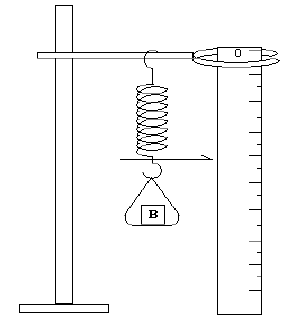
\includegraphics{./img/spring-practical.png}
\end{center}

\begin{itemize}
\item[]
\begin{itemize}
\item[(i)] Set up the apparatus as shown in the figure with zero mark of the metre-rule at the top of the rule and record the scale reading by the pointer, $S_0$.
\item[(ii)] Place the object ``B'' and standard weight (mass) W equal to 20 g in the pan and record the new pointer reading $S_1$. Calculate the extension, $e = S_1 - S_0$ in cm.
\item[(iii)] Repeat the procedure in (ii) above with W = 40 g, 60 g, 80 g and 100 g.
\end{itemize}
\item[(a)] Record your results in tabular form as shown below:\\
Table of Results:

\begin{tabular}{|p{2cm}|p{3cm}|p{3cm}|p{3cm}|}\cline{1-1}
\multicolumn{1}{|p{2cm}|}{$S_0 = $}&\multicolumn{2}{c}{} & \multicolumn{1}{p{2.5cm}}{} \\ \hline
\multicolumn{1}{|c|}{Mass} & \multicolumn{1}{c|}{Force, F (N)} & \multicolumn{1}{c|}{Pointer reading $S_1$} & \multicolumn{1}{c|}{Extension}\\
\multicolumn{1}{|c|}{(kg)} & \multicolumn{1}{c|}{} & \multicolumn{1}{c|}{(cm)} & \multicolumn{1}{c|}{$= S_1 - S_0$ (cm)}\\ \hline
\multicolumn{1}{|c|}{0} & \multicolumn{1}{c|}{} & \multicolumn{1}{c|}{} & \multicolumn{1}{c|}{}\\ 
\multicolumn{1}{|c|}{0.02} & \multicolumn{1}{c|}{} & \multicolumn{1}{c|}{} & \multicolumn{1}{c|}{}\\ 
\multicolumn{1}{|c|}{0.04} & \multicolumn{1}{c|}{} & \multicolumn{1}{c|}{} & \multicolumn{1}{c|}{}\\ 
\multicolumn{1}{|c|}{0.06} & \multicolumn{1}{c|}{} & \multicolumn{1}{c|}{} & \multicolumn{1}{c|}{}\\ 
\multicolumn{1}{|c|}{0.08} & \multicolumn{1}{c|}{} & \multicolumn{1}{c|}{} & \multicolumn{1}{c|}{}\\ 
\multicolumn{1}{|c|}{0.10} & \multicolumn{1}{c|}{} & \multicolumn{1}{c|}{} & \multicolumn{1}{c|}{}\\ \hline
\end{tabular}
\item[(b)] Plot graph of Force F (vertical axis) against extension $e$ (horizontal axis).
\item[(c)] Use your graph to evaluate
\begin{itemize}
\item[(i)] mass of B
\item[(ii)] spring constant, K, given that force, extension, constant and weight of B are related as follows:\\
F = K$e$ - B
\end{itemize}
\end{itemize}

%The aim of this experiment is to determine the mass of a given object $B$, and the
%constant of the spring provided.
%
%\begin{center}
%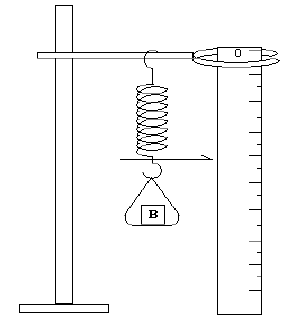
\includegraphics{./img/spring-practical.png}
%\end{center}
%
%\begin{enumerate}
%\item{Set up the apparatus as shown with the zero mark of the meter-rule at the top
%of the rule and record the scale reading, as shown by the pointer, $S_0$.}
%\item{Place the object $B$ and standard weight (mass) $W$ equal to 20~g in the pan
%and record the new pointer reading, $S_1$. Calculate the extension, $e = S_1 - S_0$ in
%cm.}
%\item{Repeat the procedure above with $W$ = 40~g, 60~g, 80~g and 100~g.}
%\item{Record your results in tabular form as shown below:
%
%\begin{center}
%\begin{tabular}{ | c | c | c | c | c | }
%\hline
%$S_0$ & Mass (kg) & Force, $F$ (N) & Pointer Reading $S_1$ (cm) & Extension, $e = S_1 - S_0$ (cm) \\ \hline
%& 0 & & & \\ \hline
%& 0.02 & & & \\ \hline
%& 0.04 & & & \\ \hline
%& 0.06 & & & \\ \hline
%& 0.08 & & & \\ \hline
%& 0.1 & & & \\ \hline
%\end{tabular}
%\end{center}
%
%}%Record your results...
%\item{Plot a graph of force $F$ (vertical axis) against extension $e$ (horizontal axis).}
%\item{Use your graph to evaluate
%\begin{enumerate}
%\item{mass of $B$}
%\item{spring constant, $K$, given that the force, extension, constant and
%weight of $B$ are related as follows: $$F = Ke - B$$}
%\end{enumerate}
%}%Use your graph...
%\end{enumerate}

\subsubsection{Discussion}

This practical has two parts: the first is to find the spring constant $k$, the second is
to find the mass of an unknown object $B$. By looking at the equation above, we
can see that $F$ is the dependent variable, $e$ is the independent variable, $K$ is the slope and
$-B$ is the intercept. When the graph is drawn, $K$ and $B$ can be found easily. Note that the
intercept on the graph will be negative.

The procedure is simply to start from a certain point on the metre rule (it does not
need to be a specific number) and to add masses one at a time, measuring the distance
from your starting point to the new position. This distance is called the extension, $e$. Be
sure that you are not simply reading the metre rule, but are measuring the distance from
the starting point.

\subsection{Simple Pendulum (Form 2)}

With some practice, this experiment should be simple for anyone to perform. The
trick comes with the math and graphing (again, an example is shown below). The
materials can all be local (string, stones, ruler) except for the stopwatches (for which you
should consult the materials section).

The practical usually has one objective: to find the acceleration due to gravity, $g$.
We know that the mass of a pendulum and its angle of deflection (for small angles) do
not affect its period. Therefore we vary only the length $L$ of the pendulum and measure
its period, as shown in the following example question.

\subsubsection{Sample Practical Question}

The aim of this experiment is to determine the magnitude of the acceleration due to
gravity, $g$. Proceed as follows:

\begin{center}
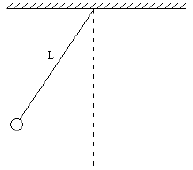
\includegraphics{./img/pendulum.png}
\end{center}


\begin{enumerate}
\item{Make a simple pendulum by suspending a weight on a string 10~cm long from a retort
stand.}
\item{Allow the pendulum to swing for twenty oscillations, using a stopwatch to record the
time. Repeat this procedure for pendulum lengths of 20~cm, 30~cm, 40~cm, and 50~cm.}
\item{Record your results in tabular form as shown below}

\begin{center}
\begin{tabular}{ | c | c | c | c | }
\hline
Pendulum Length l (m) & Time for 20 oscillations (s) & Period $T = \frac{t}{20}$ (s) & $T^2$ ($s^2$) \\ \hline
0.1 & & & \\ \hline
0.2 & & & \\ \hline
0.3 & & & \\ \hline
0.4 & & & \\ \hline
0.5 & & & \\ \hline
\end{tabular}
\end{center}

\item{Plot a graph of $T^2$ (vertical axis) against Pendulum Length (horizontal axis).}
\item{Calculate the slope of the graph.}
\item{Use the slope to calculate the value of $g$.}
\item{What are possible sources of error in this experiment?}

\end{enumerate}

\subsubsection{Discussion}

The period of a pendulum can be calculated using $$T = 2\pi\sqrt{\frac{l}{g}}$$
where $l$ is the length of the pendulum, $T$ is the period and $g$ is the acceleration due to
gravity. By squaring both sides, we get a much easier equation to graph: $$T^2 = 4\pi\frac{l}{g}$$ In this equation we see that $T^2$ is the dependent variable (y-axis) and $l$ is the
independent variable (x-axis), so the slope must be $$\mathrm{slope} = \frac{4\pi}{g}$$ 
When the graph is complete, the value of $g$ can be calculated easily.

Many students are confused by the difference between the time for many oscillations and
the period, which is the time for one oscillation. Be sure that they can change between
the two easily.

Note that pendulum practicals do not always require students to find $g$. Sometimes they are just required to find the relationship between $l$ and $t$. Again, it is essential that students read and understand the examination question, rather than memorize past solutions, and that they have lots of practice in collecting, organizing, and graphing data from a variety of experiments.

\subsection{Principle of Moments (Form 2)}

This experiment is used to verify the Principle of Moments, or equilibrium, by
balancing a meter rule on a knife-edge with masses at various distances. For this experiment, students need
a solid understanding of the Center of Gravity, the Moment of a force, and equilibrium.
Questions can range from finding the mass of an object to asking for
the mass of the metre rule. They are all
variations on the same practical: using the condition of equilibrium to find mass.

The following example is from the 2011 NECTA exam and asks students to find the mass of a battery using the Principle of Moments. Following is a brief explanation of the alternative practical of finding the mass of a metre rule.

\subsubsection{Finding the Mass of an Object}

\noindent \textbf{Sample Practical Question}\\

\noindent The aim of this experiment is to determine the mass of a given dry cell size ``AA''. Proceed as follows:
\begin{itemize}
\item[(a)] Locate and note the centre of gravity $C$ of the metre rule by balancing it on the knife edge.
\item[(b)] Suspend the 50 g mass at length `$a$' cm on one side of the metre rule and the 20 g mass together with the dry cell at length `$b$' cm on the other side of the metre rule. Fix the 50 g mass at length 30 cm from the fulcrum and adjust the position of the 20 g mass together with the dry cell until the metre rule balances horizontally. Read and record the values of $a$ and $b$ as $a_0$ and $b_0$ respectively.
\item[(c)] Draw the diagram for this experiment.
\item[(d)] By fixing $a = 5$ cm from fulcrum $C$, find its corresponding length $b$.
\item[(e)] Repeat the procedure in (d) above for $a = 10$ cm, 15 cm, 20 cm and 25 cm. Tabulate your results.
\item[(f)] Draw a graph of `$a$' against `$b$' and calculate its slope $G$.
\item[(g)] Calculate $X$ from the equation $50 = \cfrac{b_0}{a_0}(20 + X)$.
\item[(h)] Comment on the value of $\cfrac{b_0}{a_0}$.
\item[(i)] Sate the principle governing this experiment.
\end{itemize}

\noindent \textbf{Discussion}\\
This practical utilizes the Principle of Moments to find the mass of a ``AA'' battery. Initially, a known mass of 50 g is balanced with the (battery $+$ 20 g mass) system. Note that `$a$' and `$b$' are measured \emph{from the fulcrum} and so students should be careful not to just read the cm mark on the ruler where each object is suspended.

Also note that students are required to actually find the centre of gravity $C$ of the ruler rather than assuming it to be the 50 cm mark. This measured value of $C$ is to be used as the starting point for all future measurements of $a$ and $b$.

In part (g), students should recognize the equation $50 = \cfrac{b_0}{a_0}(20 + X)$ as coming from the Principle of Moments. Starting with
$$F_{\mathrm{clockwise}} \times d_{\mathrm{clockwise}} = F_{\mathrm{anticlockwise}} \times d_{\mathrm{anticlockwise}}$$
we get $$(mg)_{\mathrm{clockwise}} \times d_{\mathrm{clockwise}} = (mg)_{\mathrm{anticlockwise}} \times d_{\mathrm{anticlockwise}}$$
or $$(50 \text{g})(g) \times a_0 \text{ cm} = (20 \text{g} + X \text{g})(g) \times b_0 \text{ cm}$$
Canceling $g$ and dividing by $a_0$ reveals
$$50 = \cfrac{b_0}{a_0}(20 + X)$$
where $\cfrac{b_0}{a_0}$ is the ratio of the lever arm distances for the two weights being used. If the mass of the battery $X$ is less than 30 g, this ratio should be greater than 1, but if the mass is greater than 30 g, the ratio should be less than 1.

\subsubsection{Finding the Mass of a Metre Rule}

This question is less frequently seen on NECTA exams as compared to finding an unknown mass. However, it utilizes the same principles of equilibrium and balancing moments, and therefore is a useful alternative practical to ensure that students understand the concept rather than memorizing solutions to one version of the problem.

The mass of a uniform solid object, like a metre rule, is assumed to be at the
center of the object. In the case of the metre rule, we can say that the center of mass is at
the 50~cm mark, directly in the center. If we want it to be in equilibrium, the moments on
either side of a pivot must be equal, or $$ \mathrm{\text{Clockwise moment}} = \mathrm{\text{Anticlockwise moment}}$$
To find the mass of the metre rule itself, we begin by placing a known mass at one
point on the metre rule. We then move the pivot to one side or another until the metre
rule is perfectly balanced in equilibrium. As shown in the diagram below, the pivot will
not be at the 50~cm mark.

\begin{center}
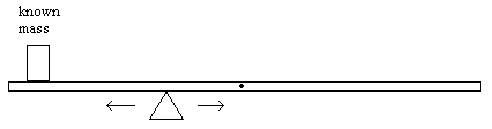
\includegraphics{./img/meter-rule.png}
\end{center}

If the metre rule is in equilibrium, we know that the moments must be equal, or
that $$F_{\mathrm{clockwise}} \times d_{\mathrm{clockwise}} = F_{\mathrm{anticlockwise}} \times d_{\mathrm{anticlockwise}}$$
In this case, the anticlockwise force is the weight of the object, and the distance is that
from the pivot to the object. The clockwise force is the weight of the metre rule, and the
distance is that from the 50~cm mark (center of mass) to the pivot. Therefore our
equation is: $$ W_{\mathrm{rule}} \times d_{\mathrm{rule}} = W_{\mathrm{object}} \times d_{\mathrm{object}} $$
Because the weight of the object is known, and the two distances can be measured, we
can easily calculate the mass and therefore the weight of the metre rule:
$$W_{\mathrm{rule}} = \frac{W_{\mathrm{object}} \times d_{\mathrm{object}}}{d_{\mathrm{rule}}}$$
From this we can calculate mass of the metre rule using $F = mg$.

%==============================================================================
\section{Light}
The light practical typically involves plane mirrors or glass blocks (rectangular
prisms). Presumably you will have already done these practicals with the students in Form
three (refraction) and Form 1 (plane mirrors), but a little practice will make the theory and
execution clear, especially if they can work in groups. The materials you will need are as
follows:
\begin{description}
\item[Cork Board]{Use cardboard for this, about 0.5 to 0.75~cm thick.}
\item[Optical pins]{Use sewing pins or syringe needles. If using syringe needs, be
sure to crimp the ends so students do not prick themselves.}
\item[Protractors]{These are cheap and students are supposed to have them anyway.
Small ones come in local mathematical sets.}
\item[Glass Block / Rectangular Prism]{A simple rectangular piece of 6~mm glass,
about 8~cm by 12~cm, will work.}
\item[Plane Mirror]{You can buy mirror glass in town in small sections for 200/= or
less; it should be available in villages through the local craftsmen if they work on
windows. Alternately, you can smoke one side of a piece of glass to make the
other side like a mirror.}
\end{description}

\subsection{Plane Mirror (Reflection) (Form 1)}

These are not as common as the rectangular prism, but they come in a variety of
questions:
\begin{itemize}
\item{Placing pins in front of a mirror at different distances and finding the distance of
the image.}
\item{Verifying the Law of Reflection at plane mirrors.}
\item{Placing two mirrors at different relative angles to find the number of images
produced.}
\end{itemize}
These are not overly complicated, but you should definitely practice with your students creating images in
mirrors -- they are not as accustomed to playing with mirrors as you might be.

Given below is an example practical from the 2006 NECTA exam which asks students to find a relationship between object distance and image distance in a plane mirror.

\subsubsection{Sample Practical Question}

Set up the experiment as shown in the diagram below using plane mirror, soft board, three pins and a white sheet of paper.

\begin{center}
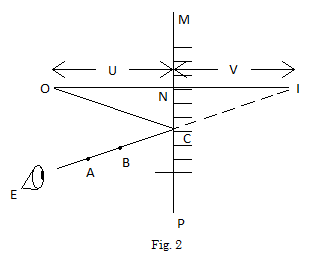
\includegraphics[width=8cm]{./img/2006-2-alt.png}
\end{center}

Fix a white sheet of paper on the soft board. Draw a line across the width at about the middle of the white sheep (MP). Draw line ONI perpendicular to MP.

Fix optical pin O to make ON = U = 3 cm. By using plasticine or otherwise, fix plane mirror along portion of MP with O in front of the mirror. With convenient position of eye, E, look into the mirror and fix optical pins A and B to be in line with image, I, of pin O.

Measure and record NI = V. Repeat procedure for U = 6 cm, 9 cm and 12 cm.

\begin{enumerate}
\item[]
\begin{enumerate}
\item[(a)] Tabulate your results as follows:

\quad \begin{tabular}{|c|c|c|c|c|} \hline
U (cm) & 3 & 6 & 9 & 12 \\ \hline
V (cm) & & & & \\ \hline
\end{tabular}

\item[(b)] Plot graph of U against V.
\item[(c)] Calculate slope, $m$ of the graph to the nearest whole number.
\item[(d)] State relationship between U and V.
\item[(e)] Write equation connecting U and V using numerical value of $m$ with symbols U and V.
\item[(f)] From your equation give position of the image when object is touching the face of the mirror.
\end{enumerate}
\end{enumerate}

\subsubsection{Discussion}
For a plane mirror, object distance and image distance are equal. That is, U and V should be approximately equal values for this practical. Note that students should extend line ONI far behind the mirror since they don't know where exactly the image I is going to be. The location of I is found at the intersection of the extended line ONI and the extended line AB connecting the two optical pins.

From the graph, the slope should be found to be 1 after rounding to the nearest whole number. From this, we can see that U = V. When the object is touching the face of the mirror, the object distance U is 0, and so the image distance V will also be 0.

\subsection{Rectangular Prism (Refraction) (Form 3)}

Students will be asked to find the refractive index and/or critical angle of the glass block by varying
the angle of incidence $i$ and measuring the corresponding angles of refraction $r$ as
described in the Mathematics section earlier. They will do this by placing two pins in
front of the prism, which together form a `ray' (the light ray), and then placing two more
pins on the other side of the prism so that, when observed through the prism from either
side, the four pins line up exactly. By drawing the lines that the pins make on the paper,
the refracted ray inside the prism can be easily traced, and the refracted angle measured.
An example question from the 2007 NECTA is given below.

\subsubsection{Sample Practical Question}

The aim of this experiment is to find the refractive index of a glass block. Proceed
as follows:\\

Place the given glass block in the middle of the drawing paper on the drawing
board. Draw lines along the upper and lower edges of the glass block. Remove the
glass block and extend the lines you have drawn. Represent the ends of these line
segments as $SS_1$ and $TT_1$. Draw the normal $NN_1$ to the parallel lines $SS_1$ and
$TT_1$ as shown in the figure below:

\begin{center}
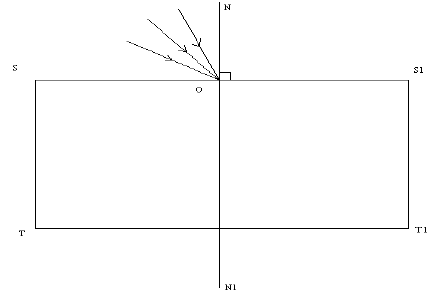
\includegraphics{./img/light-block-1.png}
\end{center}

Draw five evenly spaced lines from O to represent incident rays at different
angles of incidence (10$^\circ$, 20$^\circ$, 30$^\circ$, 40$^\circ$, and 50$^\circ$ from the normal). Replace the
glass block carefully between $SS_1$ and $TT_1$. Stick two pins $P_1$ and $P_2$ as shown in
the figure as far apart as possible along one of the lines drawn to represent an
incident ray. Locate an emergent ray by looking through the block and stick pins
$P_3$ and $P_4$ exactly in line with images $I_1$ and $I_2$ of pins $P_1$ and $P_2$. Draw the
emergent ray and repeat the procedure for all the incident rays you have drawn. Finally draw in the corresponding refracted rays.

\begin{center}
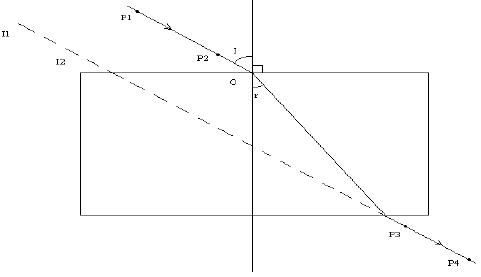
\includegraphics{./img/light-block-2.png}
\end{center}

\begin{enumerate}
\item[]
\begin{enumerate}
\item[(a)]{Record the angles of incidence $i$ and the measured corresponding angles of
refraction $r$ in a table. Your table of results should include the values of
$\sin{i}$ and $\sin{r}$.}
\item[(b)]{Plot the graph of $\sin{i}$ (vertical axis) against $\sin{r}$ (horizontal axis).}
\item[(c)]{Determine the slope of the graph.}
\item[(d)]{What is the refractive index of the glass block used?}
\item[(e)]{Mention any sources of errors in this experiment.}
\end{enumerate}
\end{enumerate}

\subsubsection{Discussion}

In this experiment, pins are used to simulate a ray of light. If all of the pins are
aligned as you look through the block, they act as a single ray. It takes practice to be able
to align the pins while looking through the block, so practice often with your students.

Light slows down as it enters a denser medium, so in order to minimize the time
required to pass through that medium, it changes direction until it moves back into its
original medium. In this case, light is moving from air into glass and then back into air,
so its direction changes while inside the glass, then returns to its original direction when
passing back into air. This effect is called refraction and it depends on the nature of the
media, in this case air and glass. Snell’s law gives us the relationship between the nature
of the media and the resulting angles of incidence and refraction:
$$n_1 \times \sin{i} = n_2 \times \sin{r}$$

In this experiment, the incident angle $i$ is being changed and the refracted angle $r$
is being measured. The refractive index of medium 1 (air) is known as 1.0, so we can use
these three to find the refractive index of medium 2 (glass). On the graph, $\sin{i}$ is the
dependent variable and $\sin{r}$ is the independent variable, so the equation becomes
$$\sin{i} = \sin{r} \frac{n_2}{n_1}$$
In this case the slope must be $\frac{n_2}{n_1}$.

The refractive index of medium air is simply 1.0, so the slope is the refractive index of
medium 2.

This practical is one of the easiest to perform with students because it does not
require much preparation. Syringe needles should be readily available and glass blocks are
cheap, so it is possible to have every students try this themselves many times before
taking the exam.

\subsubsection{Finding the Critical Angle}
Some questions may ask students to find the critical angle of a glass block in addition to its refractive index. The relationship between critical angle, $C$, and refractive index, $n$, for a particular medium is given by 
$$n = \frac{1}{\sin{C}}$$ or $$\frac{\sin{i}}{\sin{r}} = \frac{1}{\sin{C}}$$.

Thus a graph of $\sin{i}$ against $\sin{r}$ can be used to find the critical angle. However, take care to note that we must first take the reciprocal of the slope, i.e.
$$\sin{C} = \frac{1}{n}$$.

This gives us $\sin{C}$, so to get $C$ by itself, we need to use mathematical tables. Turn to the page for Natural Sines and search the table for the 4-figure value you obtained above by taking $\frac{1}{\text{slope}}$. The corresponding row gives the angle in degrees and the column gives the additional minutes of the angle.

For example, say we plot our graph of $\sin{i}$ ($y$-axis) against $\sin{r}$ ($x$-axis) and we calculate the slope to be 1.43. This is the refractive index of the glass block (since we can remember that glass has a refractive index of 1.5, we can do a quick mental check to make sure this makes sense). Then $\sin{C} = \frac{1}{1.43} = 0.6993$. From the mathematical tables, we get $C = 44^\circ 22'$ [6993 falls between 6984 ($18'$) and 6997 ($24'$), so we use the Mean Differences table to add on $4'$ giving a total of $22'$].

Note that the method of finding $n$ and $C$ changes if we are instead told to graph $\sin{r}$ ($y$-axis) against $\sin{i}$ ($x$-axis). Be sure to practice both versions with students to ensure their understanding.

%==============================================================================
\section{Electricity}

This is by far the least attempted practical on the exam, but not because it is
difficult. The electricity practical, if properly set up, is one of the easiest to perform. It
can appear in many different forms but will typically involve a simple circuit and some
kind of variable resistor in order to measure current or EMF for different resistances. The
materials you will probably need are as follows:

\begin{description}
\item[Connecting Wires]{Use speaker wire; it is cheap and available in most villages
and towns.}
\item[Voltmeters, Ammeters, Galvanometers]{This is unavoidable; you can get full
digital multimeters in town for about 10,000/=, galvanometers can be found in
any lab store or can be made using a compass and insulated copper wire.}
\item[Batteries]{Two to four D-size batteries should easily be enough for these experiments. Try to avoid Tiger brand if possible. Panasonic is highly superior in quality for roughly the same price.}
\item[Resistance Wire]{These are used to make small resistors for
the metre bridge or potentiometer. The most common type of wire to use is
nichrome, which can be found in a hardware or lab store. Steel will also work, though it
is less resistant and therefore harder to measure.}
\item[Metre Bridges]{See the activity that describes the construction of a metre bridge
and potentiometer. It is best to make both together as the construction is almost
identical and both are used frequently.}
\item[Variable Resistor (Rheostat)]{This is optional as it is typically only used to set a
level that can be easily read by the voltmeter. However, if you are using a
multimeter, you can simply change the magnitude setting on the multimeter to
account for unusually low or high resistances.}
%See How to Use a Rheostat
\item[Soldering Iron]{Not required, but may be a good investment for making reliable battery connections. Using electrical tape can lead to inconsistencies. Check large towns.}
\end{description}

\subsection{Potentiometers (Form 3)}

This experiment is very simple but requires the correct materials, namely the
meter bridge/potentiometer described above. A complete circuit is created with a switch
(optional), power source, variable resistor and 1~m of bare resistance wire, all in series.

The potentiometer itself is simple to construct; all preparation is done by the teacher, so
the student simply follows the instructions as shown in the following example from the 2007 NECTA.

\subsubsection{Sample Practical Question}

The aim of this experiment is to determine the potential fall along a uniform
resistance wire carrying a steady current. Proceed as follows:

\begin{center}
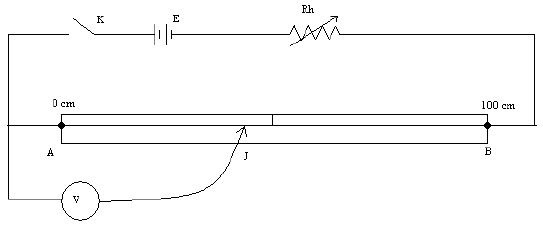
\includegraphics[width=10cm]{./img/meter-bridge-1.png}
\end{center}


Connect up the circuit as shown in the figure. Adjust the rheostat so that when the sliding
contact J is near B and the key is closed the voltmeter V indicates an almost full scale
of deflection. Do not alter the rheostat again.

Close key K and make contact with J, so that AJ = 10~cm. Record the potential
difference V volts between A and J as registered on the voltmeter.

Repeat this procedure for AJ = 20~cm, 30~cm, 50~cm, and 70~cm.

\begin{enumerate}
\item[]
\begin{enumerate}
\item[(a)]{Tabulate your results for the values of AJ and V.}
\item[(b)]{Plot a graph of V (vertical axis) against AJ (horizontal axis).}
\item[(c)]{Calculate the slope of the graph.}
\item[(d)]{What is your comment on the slope?}
\item[(e)]{State any precautions on the experiment.}
\end{enumerate}
\end{enumerate}

\subsubsection{Discussion}

This is a simple test of the relationship between the length of a wire and its
resistance, which we know is $$R=\frac{\rho l}{A} $$

Where $l$ is the length of the wire, $\rho$ is the resistivity of the wire, and $A$ is the cross-sectional
area of the wire. We expect that as the length of wire increases, its potential difference
will also increase. This is because the resistance (and therefore potential difference) of a wire is
directly related to its length. The voltmeter in this experiment is measuring just the
potential difference over the length of wire (10~cm, 20~cm, etc.), so if we use Ohm’s Law to say that $V = IR$, we can write:\\
$$ V = \frac{I \rho l}{A} $$
In this experiment, $I$, $\rho$ and $A$ are all constant, so the slope is
$$\mathrm{slope} = \frac{I \rho}{A} $$
Though it is not asked for directly in the question, we can find the resistivity, $\rho$, by measuring $I$ with an ammeter/galvanometer and $A$ with vernier calipers or a micrometer screw gauge.

\subsection{Metre Bridges (Form 3)}

A metre bridge resembles a potentiometer, except that it uses a galvanometer to
measure the difference in current between two points on the circuit, hence the name
``bridge.'' The same materials can be used as with the potentiometer, though it is best to
use small coils of resistance wire for the small resistors (between 3$\Omega$ and 20$\Omega$ is a good resistance). A galvanometer can be made easily if one is not available.

\begin{center}
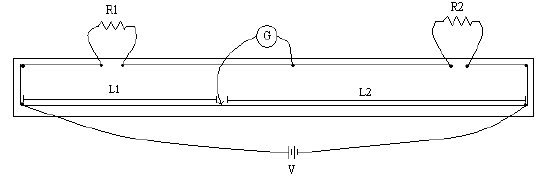
\includegraphics[width=10cm]{./img/meter-bridge-2.png}
\end{center}

Resistors $R_1$ and $R_2$ have different resistances, but they should be somehow similar so
that one resistor does not take all of the current (this will make it difficult to measure the
length to the galvanometer). About 5$\Omega$ and 10$\Omega$, for example, would work well.

However, for the sake of the practical, one resistor should not be known; the objective of
the practical is to find the unknown resistance. The long wire along the bottom edge is a
metre of nichrome wire or other resistance wire. One terminal of the galvanometer is
connected between the two resistors, and the other terminal is connected to a flying wire (or jockey)
that is free to move along the length of the nichrome wire.

The practical instructs you to move the galvanometer's flying wire back and forth
along the nichrome wire until it reads zero. At this point, we know that no current is
passing through the galvanometer, so the potential difference across it is zero. This
means that the current flowing through $R_1$ is the same as that current flowing through $R_2$,
and the current flowing through the nichrome wire is constant. From this we can
conclude that
$$ \frac{R_1}{L_1} = \frac{R_2}{L_2} $$
or that the ratio of the two resistors is equal to the ratio of distances from the flying wire
to either end of the nichrome wire. The resistance of one resistor (say, $R_1$) is known and
the lengths $L_1$ and $L_2$ can be measured from the flying wire to either side of the
nichrome wire. Using the ratio above, we can easily calculate the unknown resistance $R_2$.

An example is given below from the 2006 NECTA exam.

\subsubsection{Sample Practical Question}
You are required to determine the unknown resistance labeled X using a metre bridge circuit. Connect your circuit as shown below, where $R$ is a resistance box, G is a galvanometer, J is a jockey and others are common circuit components.

\begin{center}
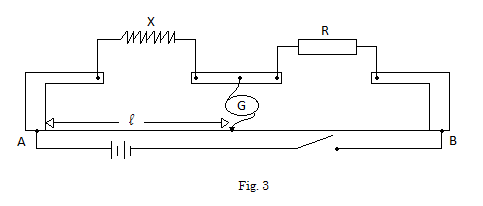
\includegraphics[width=12cm]{./img/2006-3-alt.png}
\end{center}

Procedure:\\

With $R$ = 1 $\Omega$, obtain a balance point on a metre bridge wire AB using a jockey J. Note the length $l$ in centimetres. Repeat the experiment with R equal to 2 $\Omega$, 4 $\Omega$, 7 $\Omega$ and 10 $\Omega$.\\

Tabulate your results for $R$, $l$ and $^1/_l$.

\begin{itemize}
\item[(a)]
\begin{itemize}
\item[(i)] Plot a graph of $R$ (vertical axis) against $^1/_l$ (horizontal axis).
\item[(ii)] Determine the slope S of your graph.
\item[(iii)] Using your graph, find the value of $R$ for which $^1/_l = 0.02$.
\end{itemize}
\item[(b)] Read and record the intercept $R_0$ on the vertical axis.
\item[(c)] Given that,\\
\quad \quad $R = \cfrac{100 \text{X}}{l} - \text{X}$\\
Use the equation and your graph to determine the value of X.
\item[(d)] Comment on your results in (a)(iii), (b) and (c) above.
\end{itemize}

\subsubsection{Discussion}
The procedure for this question is similar to most other wheatstone bridge problems: vary a known resistor and see how it affects the relative lengths in resistance wire required to balance the potential difference and give no current through the galvanometer. It may not be obvious at first, however, where the equation $R = \frac{100 \text{X}}{l}$ - X comes from.

Starting with the balancing ratio for a wheatstone bridge, $$ \frac{R_1}{L_1} = \frac{R_2}{L_2} $$ we can solve for the unknown resistor $$R_2 = R_1\left(\frac{L_2}{L_1}\right)$$. 

Recall that $L_1$ and $L_2$ are the corresponding lengths from either end of the metre rule to the jockey (in cm), and so taking them together, we get $$L_1 + L_2 = 100$$. Dividing both sides by $L_1$ gives $$1 + \frac{L_2}{L_1} = \frac{100}{L_1}$$. Then solving for $\frac{L_2}{L_1}$, $$\frac{L_2}{L_1} = \frac{100}{L_1} - 1$$. Now substitute this into our previous equation for $R_2$: $$R_2 = R_1\left(\frac{100}{L_1} - 1\right)$$. Replacing $R_2$ with $R$, $L_1$ with $l$ and $R_1$ with X for this problem and distributing gives, $$R = \frac{100 \text{X}}{l} - \text{X}$$.

From this equation, we have dependent variable $R$, independent variable $\frac{1}{l}$, slope $100 \text{X}$ and $y$-intercept $-\text{X}$. So we can obtain the value of the unknown resistor X either by using the $y$-intercept (note the resistance is a positive value) or by taking the slope divided by 100.

\subsection{Ohm’s Law (Form 2)}

The practical may give any kind of experiment to use or verify Ohm’s Law in a
simple circuit. Finding the e.m.f. and internal resistance of cells appears frequently. Students should be very familiar with the law, as well as the factors that determine resistance in a wire and the effect of internal resistance of a cell on a circuit. Given below is an example problem taken from the 2011 NECTA exam.

\subsubsection{Sample Practical Question}
You are provided with an ammeter, A, resistance box, R, dry cell, D, a key, K and connecting wires. Proceed as follows:
\begin{enumerate}
\item[]
\begin{enumerate}
\item[(a)] Connect the circuit in series.
\item[(b)] Put $R$ = 1 $\Omega$ and quickly read the value of current $I$ on the ammeter.
\item[(c)] Repeat procedure (b) above for $R$ = 2 $\Omega$, 3 $\Omega$, 4 $\Omega$ and 5 $\Omega$. Record your results in a tabular form.
\item[(d)] Draw the circuit diagram for this experiment.
\item[(e)] Plot the graph of $R$ against $\cfrac{1}{I}$.
\item[(f)] Determine the slope of the graph.
\item[(g)] If the graph obeys the equation $R=\cfrac{E}{I}-r$, then
\begin{enumerate}
\item[(i)] suggest how $E$ and $r$ may be evaluated from your graph.
\item[(ii)] compute $E$.
\item[(iii)] compute $r$.
\end{enumerate}
\item[(h)] State one source of error and suggest one way of minimizing it.
\item[(i)] Suggest the aim of this experiment.
\end{enumerate}
\end{enumerate}

\subsubsection{Discussion}
To see where the equation $R=\cfrac{E}{I}-r$ comes from, first start with Ohm's Law, $V = IR$. Accounting for the internal resistance of the cell, $r$, this becomes $$V = I(R + r)$$. To solve for resistance, we divide both sides by $I$, which gives $$(R + r) = \frac{V}{I}$$. From this we can see that, using $E$ as e.m.f. for this problem, $$R=\cfrac{E}{I}-r $$. 

In this form, the equation resembles the classic $y = mx + c$, where $R$ is the dependent variable, $\frac{1}{I}$ the independent variable, $E$ is the slope and $-r$ is the y-intercept (note the internal resistance is a positive value).

%\pagebreak
%
%\section{NECTA Past Papers}
%\setcounter{secnumdepth}{1}
%\subsection{2011 - PHYSICS 2A ACTUAL PRACTICAL A}

\begin{enumerate}
\item The aim of this experiment is to determine the mass of a given dry cell size ``AA''. Proceed as follows:
\begin{itemize}
\item[(a)] Locate and note the centre of gravity $C$ of the metre rule by balancing it on the knife edge.
\item[(b)] Suspend the 50 g mass at length `$a$' cm on one side of the metre rule and the 20 g mass together with the dry cell at length `$b$' cm on the other side of the metre rule. Fix the 50 g mass at length 30 cm from the fulcrum and adjust the position of the 20 g mass together with the dry cell until the metre rule balances horizontally. Read and record the values of $a$ and $b$ as $a_0$ and $b_0$ respectively.
\item[(c)] Draw the diagram for this experiment.
\item[(d)] By fixing $a = 5$ cm from fulcrum $C$, find its corresponding length $b$.
\item[(e)] Repeat the procedure in (d) above for $a = 10$ cm, 15 cm, 20 cm and 25 cm. Tabulate your results.
\item[(f)] Draw a graph of `$a$' against `$b$' and calculate its slope $G$.
\item[(g)] Calculate $X$ from the equation $50 = \cfrac{b_0}{a_0}(20 + X)$.
\item[(h)] Comment on the value of $\cfrac{b_0}{a_0}$.
\item[(i)] Sate the principle governing this experiment.
\end{itemize}
\end{enumerate}

\flushright \textbf{(25 marks)}
\begin{enumerate}
\item[2.] You are provided with an ammeter, A, resistance box, R, dry cell, D, a key, K and connecting wires. Proceed as follows:
\begin{enumerate}
\item[(a)] Connect the circuit in series.
\item[(b)] Put $R$ = 1 $\Omega$ and quickly read the value of current $I$ on the ammeter.
\item[(c)] Repeat procedure (b) above for $R$ = 2 $\Omega$, 3 $\Omega$, 4 $\Omega$ and 5 $\Omega$. Record your results in a tabular form.
\item[(d)] Draw the circuit diagram for this experiment.
\item[(e)] Plot the graph of $R$ against $\cfrac{1}{I}$.
\item[(f)] Determine the slope of the graph.
\item[(g)] If the graph obeys the equation $R=\cfrac{E}{I}-r$, then
\begin{enumerate}
\item[(i)] suggest how $E$ and $r$ may be evaluated from your graph.
\item[(ii)] compute $E$.
\item[(iii)] compute $r$.
\end{enumerate}
\item[(h)] State one source of error and suggest one way of minimizing it.
\item[(i)] Suggest the aim of this experiment.
\end{enumerate}

\end{enumerate}

\flushright \textbf{(25 marks)}
\flushleft
%\pagebreak
%\section{2010 - PHYSICS 2A ALTERNATIVE A PRACTICAL}

\begin{enumerate}
\item[1.] The aim of this experiment is to find the mass of the unknown load labeled ``$W$'' and the spring constant $K$. Proceed as follows:

\begin{center}
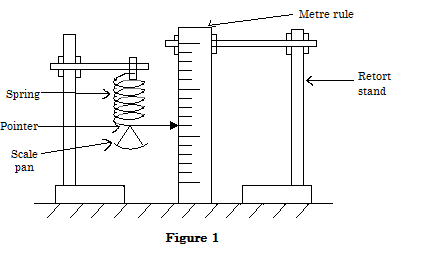
\includegraphics[width=14cm]{./img/2010-1-alt.png}
\end{center}

Set up the apparatus as shown in Figure 1. Put a mass of 50 g on the scale pan and record the equilibrium position $X_0$ of the pointer. Put on the scale pan the unknown weight marked $W$. Without removing $W$ and the 50 g mass in the scale pan, add a load $L$ of 50 g and record the new position of the pointer $X$. Calculate the extension $E = (X - X_0)$. Repeat this process for $L$ = 100 g, 150 g, 200 g and 250 g.
\begin{enumerate}
\item[(a)] Record you conclusions as shown in Table 1.\\[10pt]

Equilibrium position $X_0$..................\\[10pt]

Table 1\\[10pt]

%\begin{center}
\begin{tabular}{|p{3cm}|p{3cm}|p{3cm}|} \hline
\multicolumn{1}{|c|}{Load (g)} & \multicolumn{1}{c|}{$X$ (cm)} & \multicolumn{1}{c|}{$E = X - X_0$ (cm)} \\ \hline
\multicolumn{1}{|c|}{50} & & \\ \hline
\multicolumn{1}{|c|}{100} & & \\ \hline
\multicolumn{1}{|c|}{150} & & \\ \hline
\multicolumn{1}{|c|}{200} & & \\ \hline
\multicolumn{1}{|c|}{250} & & \\ \hline
\end{tabular}\\[10pt]
%\end{center}

\item[(b)] Plot the graph of load L against absolute value of extension E. The scale of the vertical axis should be chosen to range from 200 g to 300 g.
\item[(c)] From the graph, determine the unknown weight marked W, given that L = KE + W where K is a constant.
\item[(d)] What does the gradient of the graph represent?
\item[(e)] State the sources of errors and precautions that should be taken in the experiment.
\end{enumerate}
\end{enumerate}
\flushright \textbf{(25 marks)}

\pagebreak

\begin{enumerate}
\item[2.] The aim of this experiment is to determine the refractive index of water. Proceed as follows:

\begin{center}
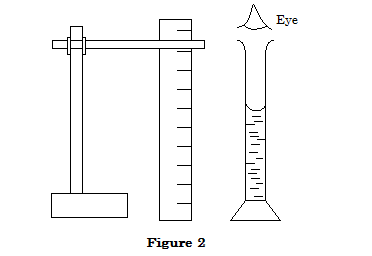
\includegraphics[width=10cm]{./img/2010-2-alt.png}
\end{center}

\begin{enumerate}
\item[(a)] Arrange your apparatus as in Figure 2. Put about 150 cm$^3$ of clear water in the measuring cylinder. Drop an office pin at the bottom so that it rests touching the wall of the cylinder.
\item[(b)] Look in the cylinder from Figure 2. Use another office pin as a search pin, move it up and down outside the cylinder, and locate the image position by no parallax method. Locate the image position of the ruler. Measure and record the depth ($H_1$) of the image. Measure and record the depth ($H_2$) of water. Repeat the experiment with 175 cm$^3$, 200 cm$^3$, 225 cm$^3$ and 250 cm$^3$ of water in the measuring cylinder.
\item[(c)] 
\begin{enumerate}
\item[(i)] Record in Table 2 your values of $H_1$ and $H_2$ corresponding to the volumes of water in the measuring cylinder.\\[10pt]

Table 2\\[10pt]

%\begin{center}
\begin{tabular}{|p{3cm}|p{3cm}|p{3cm}|} \hline
\multicolumn{1}{|c|}{Volume of water V (cm)} & \multicolumn{1}{c|}{$H_1$} & \multicolumn{1}{c|}{$H_2$} \\ \hline
\multicolumn{1}{|c|}{150} & & \\ \hline
\multicolumn{1}{|c|}{175} & & \\ \hline
\multicolumn{1}{|c|}{200} & & \\ \hline
\multicolumn{1}{|c|}{225} & & \\ \hline
\multicolumn{1}{|c|}{250} & & \\ \hline
\end{tabular}\\[10pt]
%\end{center}

\item[(ii)] Plot the graph of $H_2$ versus $H_1$.
\item[(iii)] Determine the slope of the graph.
\item[(iv)] What is the physical meaning of the slope?
\item[(v)] State sources of error in this experiment.
\end{enumerate}
\end{enumerate}
\end{enumerate}
\flushright \textbf{(25 marks)}

\pagebreak

\begin{enumerate}
\item[3.] The aim of this experiment is to determine the resistivity of an electrical conductor $P$.

\begin{center}
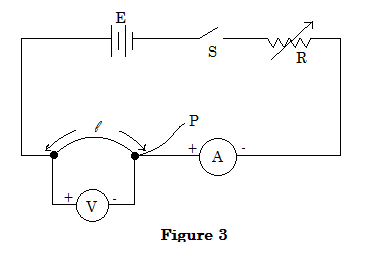
\includegraphics[width=10cm]{./img/2010-3-alt.png}
\end{center}

With $P$ having a length $l = 50$ cm, connect up the circuit as shown in Figure 3. Close one key S and adjust the rheostat R so that the current in $P$ is 0.20 A. Record the current $I$ and the potential difference $V$ between its ends.\\[10pt]

Repeat the procedure with current $I = $0.30 A, 0.40 A, 0.50 A and 0.60 A.
\begin{enumerate}
\item[(a)] Record your results in Table 3.\\[10pt]

Table 3\\[10pt]

%\begin{center}
\begin{tabular}{|p{3cm}|p{3cm}|} \hline
\multicolumn{1}{|c|}{Current $I$ (A)} & \multicolumn{1}{c|}{P.d. (volts)} \\ \hline
\multicolumn{1}{|c|}{0.20} &  \\ \hline
\multicolumn{1}{|c|}{0.30} &  \\ \hline
\multicolumn{1}{|c|}{0.40} &  \\ \hline
\multicolumn{1}{|c|}{0.50} &  \\ \hline
\multicolumn{1}{|c|}{0.60} &  \\ \hline
\end{tabular}\\[10pt]
%\end{center}

\item[(b)] Plot a graph of $V$ against $I$ and calculate the slope $G$.
\item[(c)] Deduce the resistivity of the conductor $P$ given that; $\rho = \cfrac{G\pi d^2}{4l}$.\\[10pt]
Where $\rho$ = resistivity\\
$d$ = diameter of $P$ (measured using the micrometer screw gauge provided).
\end{enumerate}
\end{enumerate}

\flushright \textbf{(25 marks)}
\flushleft
%\pagebreak
%\subsection{2009 - PHYSICS 2A ALTERNATIVE A PRACTICAL}

\begin{enumerate}
\item[1.] In this experiment you are required to find the relationship between the length of a simple pendulum and its period. Proceed as follows:
\begin{itemize}
\item[(a)] Suspend a simple pendulum of length L = 100 cm. Displace the pendulum through a small angle so that it swings parallel to the edge of the bench or table, determine the time for 20 oscillations. Continue reducing the length of the pendulum by 10 cm each time and obtain a total of six readings.
\item[(b)] Record your readings in a table as shown below.


\begin{tabular}{|p{2.5cm}|p{2.5cm}|p{2.5cm}|p{2.5cm}|p{2.5cm}|} \hline
Length of pendulum L (cm) & Log$_{10}$L & Time for 20 oscillations & Period T & Log$_{10}$T \\ \hline
&&&& \\ 
&&&& \\ 
&&&& \\ 
&&&& \\ 
&&&& \\ 
&&&& \\ 
&&&& \\ 
&&&& \\ \hline
\end{tabular}\\[10pt]

\noindent Assuming that T $ \propto $ L$^a$, we have T = $k$L$^a$ and taking logarithms to base ten on both sides we get $\log_{10}$T = $a\log_{10}$L + $\log_{10}k$.

\begin{itemize}
\item[(i)] Plot a graph of $\log_{10}$T (vertical axis) against $\log_{10}$L (horizontal axis) hence determine the values of $a$ and $k$ each correct to one decimal place.
\item[(ii)] From your answer in (i) above write down the values of $a$ and $k$ each in the form of $\cfrac{b}{c}$ where $b$ and $c$ are integers (i.e. whole numbers).
\item[(iii)] From the assumption and your answer in (ii) deduce the form of the equation governing the motion of the simple pendulum.
\end{itemize}

\end{itemize}
\end{enumerate}
\flushright \textbf{(25 marks)}


\begin{enumerate}
\item[2.] The aim of this experiment is to determine the refractive index $\eta$ of a given glass block.

\begin{center}
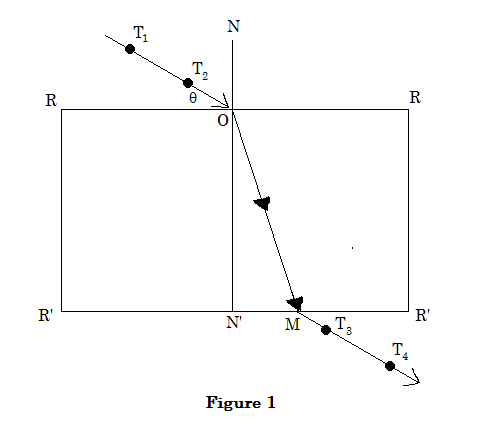
\includegraphics[width=8cm]{./img/2009-2-alt.png}
\end{center}

Place the rectangular glass block on the white paper on a drawing board. Using a pencil trace the outline of the block. Remove the glass block and draw a normal NOM near the left end of the block (Figure 1).\\[10pt]

\noindent Using a protractor and a pencil measure $\theta = 20^\circ$, draw a line making the angle $20^\circ$ with the surface RR of the block. Erect two pins T$_1$ and T$_2$ on this line and at a suitable distance from one another. Return the block and erect the pins T$_3$ and T$_4$ at positions such that they lie in a straight line with pins T$_1$ and T$_2$ as seen through the block. Now remove the block and draw a complete path of the ray (Figure 1).\\[10pt]

\noindent Measure the length MN$'$ and ON$'$: Repeat the procedure for values of $\theta = 30^\circ, 40^\circ$ and $60^\circ$ respectively. In each case make a drawing on a fresh part of the drawing paper.

\begin{itemize}
\item[(a)] Record the values of $\theta$, MN$'$, ON$'$, $\cfrac{\text{MN}'}{\text{ON}'}$ and $\cos \theta$ in a tabular form.
\item[(b)] Plot a graph of $\cfrac{\text{MN}'}{\text{ON}'}$ against $\cos \theta$.
\item[(c)] Find the slope $G$ of the graph.
\item[(d)] Calculate the value of the refractive index $\eta$; given that $G = \cfrac{1}{\eta}$.
\item[(e)] State two sources of errors. \hfill \textbf{(25 marks)}
\end{itemize}

\end{enumerate}


\begin{enumerate}
\item[3.] The aim of this experiment is to verify Ohm's Law.

\begin{center}
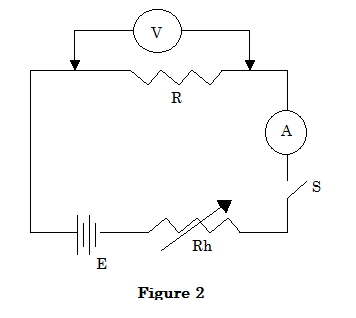
\includegraphics[width=7cm]{./img/2009-3-alt.png}
\end{center}

\begin{itemize}
\item[(a)] Set up the apparatus as shown on Figure 2, close switch S. Adjust the Rheostat Rh by sliding slowly from one end, read and record the value V of the voltmeter and current I of the ammeter.
\item[(b)] Repeat the experiment by changing the Rheostat slider to obtain about five pair of readings.\\[10pt]

\textbf{NB:} Adjust the Rheostat until when the pointer is exactly on the division of the metre scale.\\[10pt]

Table of results\\[10pt]
\begin{tabular}{|c|c|c|c|c|c|c|c|}\hline
V (V)&&&&&&&\\ \hline
I (A)&&&&&&& \\ \hline
\end{tabular}

\item[(c)] Plot a graph of V (vertical axis) against I (horizontal axis).
\item[(d)] 
\begin{itemize}
\item[(i)] Find the slope of the graph.
\item[(ii)] What is the relation between V and I?
\item[(iii)] Find the resistance R. \hfill \textbf{(25 marks)}
\end{itemize}
\end{itemize}

\end{enumerate}
\flushleft

%\pagebreak
%\section{2007 - PHYSICS 2A ALTERNATIVE A PRACTICAL}

\begin{enumerate}
\item[1.] The aim of this experiment is to determine the mass of a given object ``B'', and the constant of the spring provided.

\begin{center}
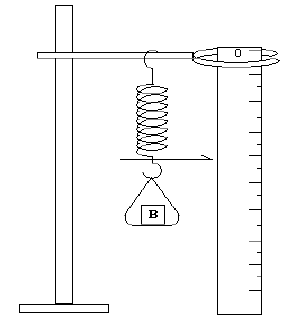
\includegraphics[width=7cm]{./img/2007-1-alt.png}
\end{center}

\begin{itemize}
\item[]
\begin{itemize}
\item[(i)] Set up the apparatus as shown in Fig. 1 with zero mark of the metre-rule at the top of the rule and record the scale reading by the pointer, $S_0$.
\item[(ii)] Place the object ``B'' and standard weight (mass) W equal to 20 g in the pan and record the new pointer reading $S_1$. Calculate the extension, $e = S_1 - S_0$ in cm.
\item[(iii)] Repeat the procedure in (ii) above with W = 40 g, 60 g, 80 g and 100 g.
\end{itemize}
\item[(a)] Record your results in tabular form as shown below:\\
Table of Results:

\begin{tabular}{|p{2cm}|p{3cm}|p{3cm}|p{3cm}|}\cline{1-1}
\multicolumn{1}{|p{2cm}|}{$S_0 = $}&\multicolumn{2}{c}{} & \multicolumn{1}{p{2.5cm}}{} \\ \hline
\multicolumn{1}{|c|}{Mass} & \multicolumn{1}{c|}{Force, F (N)} & \multicolumn{1}{c|}{Pointer reading $S_1$} & \multicolumn{1}{c|}{Extension}\\
\multicolumn{1}{|c|}{(kg)} & \multicolumn{1}{c|}{} & \multicolumn{1}{c|}{(cm)} & \multicolumn{1}{c|}{$= S_1 - S_0$ (cm)}\\ \hline
\multicolumn{1}{|c|}{0} & \multicolumn{1}{c|}{} & \multicolumn{1}{c|}{} & \multicolumn{1}{c|}{}\\ 
\multicolumn{1}{|c|}{0.02} & \multicolumn{1}{c|}{} & \multicolumn{1}{c|}{} & \multicolumn{1}{c|}{}\\ 
\multicolumn{1}{|c|}{0.04} & \multicolumn{1}{c|}{} & \multicolumn{1}{c|}{} & \multicolumn{1}{c|}{}\\ 
\multicolumn{1}{|c|}{0.06} & \multicolumn{1}{c|}{} & \multicolumn{1}{c|}{} & \multicolumn{1}{c|}{}\\ 
\multicolumn{1}{|c|}{0.08} & \multicolumn{1}{c|}{} & \multicolumn{1}{c|}{} & \multicolumn{1}{c|}{}\\ 
\multicolumn{1}{|c|}{0.10} & \multicolumn{1}{c|}{} & \multicolumn{1}{c|}{} & \multicolumn{1}{c|}{}\\ \hline
\end{tabular}
\item[(b)] Plot graph of Force F (vertical axis) against extension $e$ (horizontal axis).
\item[(c)] Use your graph to evaluate
\begin{itemize}
\item[(i)] mass of B
\item[(ii)] spring constant, K, given that force, extension, constant and weight of B are related as follows:\\
F = K$e$ - B
\end{itemize}
\end{itemize}

\end{enumerate}
\flushright \textbf{(25 marks)}



\begin{enumerate}
\item[2.] The aim of this experiment is to find the refractive index of a glass block. Proceed as following:\\[10pt]

Place the given glass block in the middle of the drawing paper on the drawing board. Draw lines along the upper and lower edge of the glass block. Remove the glass block and extend the line you have drawn. Represent the ends of those line segments as SS$^1$ and TT$^1$. Draw the normal NN$^1$ to the parallel lines SS$^1$ and TT$^1$ as shown in Fig. 2(a).

\begin{center}
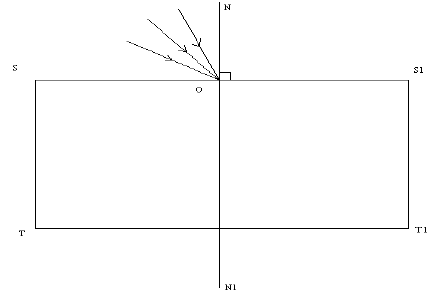
\includegraphics[width=8cm]{./img/2007-2a-alt.png}
\end{center}

Draw five evenly spaced lines from O to represent incident rays at different angles of incidence (10$^\circ$, 20$^\circ$, 30$^\circ$, 40$^\circ$ and 50$^\circ$ from the normal). Replace the glass block carefully between SS$^1$ and TT$^1$. Stick two pins P$_1$ and P$_2$ as shown in Fig. 2(b) as far apart as possible along one of the lines drawn to represent an incident ray. Locate an emergent ray by looking through the block and stick pins P$_3$ and P$_4$ exactly in line with images I$_1$ and I$_2$ of pins P$_1$ and P$_2$. Draw the emergent ray and repeat the procedure for all the incident rays you have drawn. Finally draw in the corresponding refracted rays.\\[10pt]

NOTE: The drawing paper should be handed in together with other answer sheets.

\begin{center}
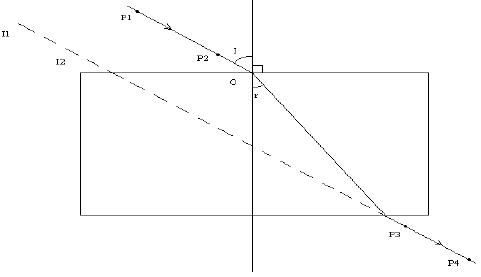
\includegraphics[width=10cm]{./img/2007-2b-alt.png}
\end{center}

\begin{itemize}
\item[(a)] Record the angles of incidence I and the measured corresponding angles of refraction ``r'' in a table. Your table of results should include the values of $\sin$ I and $\sin$ r.
\item[(b)] Plot the graph of $\sin$ I (vertical - axis) against $\sin$ r (horizontal - axis).
\item[(c)] Determine the slope of the graph.
\item[(d)] What is the refractive index of the glass block used?
\item[(e)] Mention any sources of errors in this experiment.
\end{itemize}

\end{enumerate}
\flushright \textbf{(25 marks)}


\begin{enumerate}
\item[3.] The aim of this experiment is to determine the potential fall along a uniform resistance wire carrying a steady current.\\[10pt]

Proceed as follows:

\begin{center}
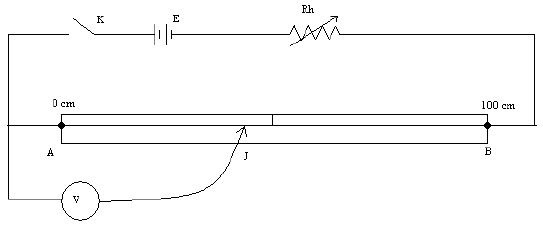
\includegraphics[width=12cm]{./img/2007-3-alt.png}
\end{center}

Connect up the circuit as shown in Fig. 3. Adjust the rheostat so that when the sliding contact J is near B, and the key is closed the voltmeter V indicates an almost full scale deflection. Do not alter the rheostat again.\\

Close key K and make contact with J, so that AJ = 10 cm. Record the potential different V volts between A and J as registered on the voltmeter.\\

Repeat this procedure for AJ = 20 cm, 30 cm, 50 cm and 70 cm.

\begin{itemize}
\item[(a)] Tabulate your results for the values of AJ and V.
\item[(b)] Plot a graph of V (vertical axis) against AJ (horizontal axis).
\item[(c)] Calculate the slope of the graph.
\item[(d)] What is your comment on the slope?
\item[(e)] State any precautions on the experiment.
\end{itemize}

\end{enumerate}
\flushright \textbf{(25 marks)}
\flushleft
%\pagebreak
%\section{2006 - PHYSICS 2A ALTERNATIVE A PRACTICAL}

\begin{enumerate}
\item[1.] In this experiment you are required to determine the mass of unknown object ``X''.

\begin{center}
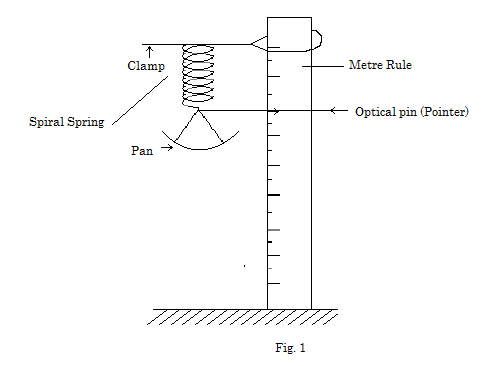
\includegraphics[width=10cm]{./img/2006-1-alt.png}
\end{center}

Assemble the pieces of apparatus as shown in Figure 1, with zero mark scale of the rule at the lower most end.\\

Record the reading of the position of pointer on the scale of metre-rule when the pan is empty as $S_0$.\\

Put 20 g to the pan and record pointer reading $S$.\\

Find extension $e = S - S_0$ cm.\\

Repeat the procedure for mass of 40 g, 60 g, 80 g and 100 g. Put object X on the pan and record its pointer reading.

\begin{itemize}
\item[(a)] Summarize your results in a table as follows:\\[10pt]
\begin{center}
\begin{tabular}{|l|c|c|c|c|c|c|} \hline
Mass on pan (g) &20&40&60&80&100&X \\ \hline
Pointer reading (cm) &&&&&& \\ \hline
Extension, $e = S - S_0$ (cm) &&&&&& \\ \hline
\end{tabular} \\[10pt]
\end{center}
\item[(b)] Plot graph of mas against extension (m Vs. $e$).
\item[(c)] Find slope, P, of your graph.
\item[(d)] Find mass X.
\item[(e)] Find Q, given that Q = P $\times$ $e_\text{x}$, where $e_\text{x}$ is extension of X.
\item[(f)] Comment on Q and X.
\end{itemize}


\end{enumerate}

\begin{enumerate}
\item[2.] Set up the experiment as shown in the diagram below using plane mirror, soft board, three pins and a white sheet of paper.

\begin{center}
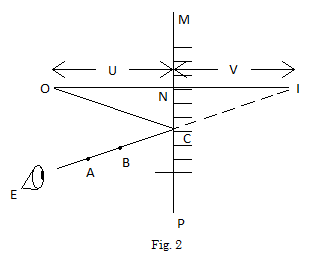
\includegraphics[width=6cm]{./img/2006-2-alt.png}
\end{center}

Fix a white sheet of paper on the soft board. Draw a line across the width at about the middle of the white sheep (MP). Draw line ONI perpendicular to MP.\\

Fix optical pin O to make ON = U = 3 cm. By using plasticine or otherwise, fix plane mirror along portion of MP with O in front of the mirror. With convenient position of eye, E, look into the mirror and fix optical pins A and B to be in line with image, I, of pin O.\\

Measure and record NI = V. Repeat procedure for U = 6 cm, 9 cm and 12 cm.

\begin{itemize}
\item[(a)] Tabulate your results as follows:\\[10pt]

\quad \quad \begin{tabular}{|l|c|c|c|c|} \hline
U (cm) &3&6&9&12 \\ \hline
V (cm) &&&& \\ \hline
\end{tabular} \\[10pt]

\item[(b)] Plot graph of U against V.
\item[(c)] Calculate slope, m, of the graph to the nearest whole number.
\item[(d)] State relationship between U and V.
\item[(e)] Write equation connecting U and V using numerical value of m with symbols U and V.
\item[(f)] From your equation give position of the image when object is touching the face of the mirror.
\end{itemize}

\end{enumerate}


\begin{enumerate}
\item[3.] You are required to determine the unknown resistance labeled X using a metre bridge circuit. Connect your circuit as shown below, where R is a resistance box, G is a galvanometer, J is a jockey and others are common circuit components.

\begin{center}
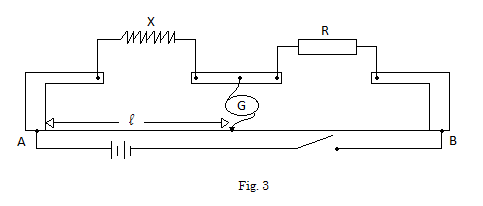
\includegraphics[width=14cm]{./img/2006-3-alt.png}
\end{center}

Procedure:\\

With R = 1 $\Omega$, obtain a balance point on a metre bridge wire AB using a jockey J. Note the length $l$ in centimetres. Repeat the experiment with R equal to 2 $\Omega$, 4 $\Omega$, 7 $\Omega$ and 10 $\Omega$.\\

Tabulate your results for R, $l$ and $^1/_l$.

\begin{itemize}
\item[(a)]
\begin{itemize}
\item[(i)] Plot a graph of R (vertical axis) against $^1/_l$ (horizontal axis).
\item[(ii)] Determine the slope S of your graph.
\item[(iii)] Using your graph, find the value of R for which $^1/_l = 0.02$.
\end{itemize}
\item[(b)] Read and record the intercept R$_0$ on the vertical axis.
\item[(c)] Given that,\\
\quad \quad R = $\cfrac{100\text{X}}{l}$ - X\\
Use the equation and your graph to determine the value of X.
\item[(d)] Comment on your results in (a)(iii), (b) and (c) above.
\end{itemize}

\end{enumerate}
%\pagebreak
%\subsection{2005 - PHYSICS 2A ALTERNATIVE A PRACTICAL}

\begin{enumerate}
\item[1.] The aim of this experiment is to determine the mass of unknown weight labelled \textbf{X} and the force constant of the spring \textbf{k}.

\begin{center}
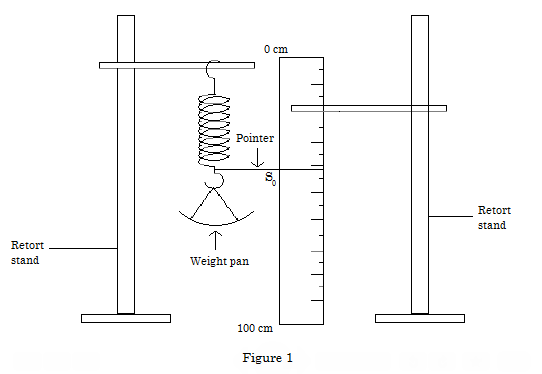
\includegraphics[width=12cm]{./img/2005-1-alt.png}
\end{center}

Set up the apparatus provided as shown in figure 1 above. Add 50 g mass on to the weight pan so that any ``kinks'' in the spring are removed. Leave this weight for the whole experiment but ignore it in all readings. Record the scale reading $S_0$. Add 50 g on to the weight pan and record the new scale reading $S$. Calculate the extension ($e = S - S_0$) caused by the weight. Repeat with different weights ($W$) to obtain at least five readings. Tabulate your results. Replace the weights ($W$) by the weight \textbf{X} provided and find the corresponding extension.\\[10pt]

Record this extension as $S_{\text{X}}$ ............. cm

\begin{enumerate}
\item[(a)] Plot a graph of load against extension.
\item[(b)]
\begin{enumerate}
\item[(i)] Find the gradient (G) of your graph.
\item[(ii)] What is the physical meaning of the gradient?
\end{enumerate}
\item[(c)] From the graph, what is the mass of the weight labelled \textbf{X}?
\end{enumerate}

\item[2.] The aim of this experiment is to find the critical angle \textbf{C} of the given glass block.

\begin{center}
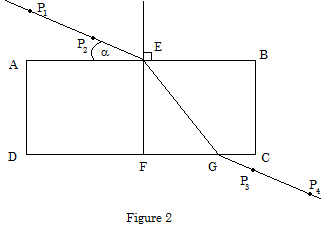
\includegraphics[width=10cm]{./img/2005-2-alt.png}
\end{center}

\textbf{Proceed as follows:}\\[10pt]

Place a white sheet of paper on the drawing board. Place the glass block, with one of its largest surfaces top most on top of the white paper. Mark the outline of the glass block on the paper with a pencil. Then remove the glass block and draw a line which cuts its largest sides normally at E and F as shown in figure 2 above. \\[10pt]

Using a protractor draw an angle $\alpha = 30^\circ$ with the glass block. Replace the glass block in its original position and stick the first pin P$_1$ and second pin P$_2$ along the line of angle $\alpha = 30^\circ$. Stick the third and fourth pins P$_3$ and P$_4$ respectively on the opposite side of the glass block such that P$_3$ and P$_4$ fall on a straight line with P$_1$ and P$_2$ when viewed through side CD of the glass block. \\[10pt]

Remove the glass block and trace the straight path taken by the ray G P$_3$ P$_4$. Using a ruler, join G and E. \\[10pt]

Measure the angle of refraction $r^\circ$, then calculate the values of $\cos{\alpha}$ and $\sin{r^\circ}$. Repeat the same procedure for values $\alpha = 40^\circ$, $50^\circ$, $60^\circ$, $70^\circ$ and $80^\circ$. Record your results in tabular form for the values of $\alpha$, $r^\circ$, $\sin{r^\circ}$ and $\cos{\alpha}$.

\begin{enumerate}
\item[(a)] Plot a graph of $\sin{r^\circ}$ (vertical axis) against $\cos{\alpha}$ (horizontal axis).
\item[(b)] Find the slope of the graph.
\item[(c)] Calculate the value of $C$ where slope = $\sin{C}$.
\item[(d)] State the possible sources of error and precautions you have taken during the experiment.
\end{enumerate}

\item[3.] The aim of this experiment is to determine the \textbf{e.m.f. E} and internal resistance \textbf{r} of a cell.

\begin{center}
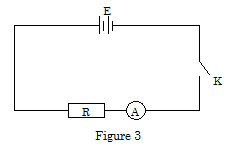
\includegraphics[width=7cm]{./img/2005-3-alt.png}
\end{center}

\begin{enumerate}
\item[(a)] Connect the circuit as shown in figure 3 above. Put $R = 1 \Omega$ and quickly read the value of $i$ on the ammeter.
\item[(b)] Repeat the procedure in 3 (a) above, for values of $R = 2 \Omega$, $3 \Omega$, $4 \Omega$ and $5 \Omega$ respectively.
\item[(c)] Tabulate your results and complete the following table.
\begin{center}
\begin{tabular}{|c|c|c|} \hline
\textbf{Resistance $R$ ($\Omega$)} & \textbf{Current $i$ (A)} & \textbf{$\cfrac{1}{i} \left(\text{A}^{-1}\right)$ } \\ \hline
1&& \\
2&& \\
3&& \\
4&& \\
5&& \\ \hline
\end{tabular} \\[10pt]
\end{center}
\item[(d)] Plot the graph of $R$ against $\cfrac{1}{i}$.
\item[(e)] The graph uses the equation $R = \cfrac{E}{i} - r$.
\begin{enumerate}
\item[(i)] Suggest how $E$ and $r$ may be evaluated from your graph.
\item[(ii)] Evaluate $E$ for one cell.
\item[(iii)] Evaluate $r$ for one cell.
\end{enumerate}
\item[(f)] State one source of error and suggest one way of minimizing it.
\end{enumerate}

\end{enumerate}
%\pagebreak
%\subsection{2004 - PHYSICS 2A ALTERNATIVE A PRACTICAL}

\begin{enumerate}
\item[1.] The aim of this experiment is to determine the mass of a given dry cell, size ``AA''.\\[5pt]

You are provided with a dry cell, a knife edge, two weights 50 g and 20 g, and a metre rule.\\[5pt]

Proceed as follows:
\begin{enumerate}
\item[(a)] Locate and note the centre of gravity C of the metre rule by balancing on the knife edge.
\item[(b)] Suspend the 50 g mass on one side of the metre rule, and 20 g together with the dry cell on the other side of the metre rule adjusting their position until the metre rule balances horizontally, as shown in Figure 1 below.

\begin{center}
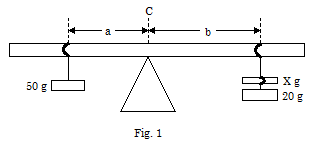
\includegraphics[width=10cm]{./img/2004-1-alt.png}
\end{center}

\item[(c)] By fixing a = 5 cm from C find its corresponding length, b, from C.
\item[(d)] Repeat and tabulate your results using a = 10 cm, 15 cm, 20 cm and 25 cm.
\item[(e)] Draw a graph of ``a'' against ``b'' and calculate its slope G.
\item[(f)] Calculate X from the equation $\text{G} = \cfrac{20 + \text{X}}{50}$. \hfill \textbf{(25 marks)}
\end{enumerate}


\item[2.] You are provided with a glass block, drawing board, optical pins and plane papers.\\

Place a white piece of paper on the drawing board. Place the glass block with one of its largest surface top most on top of the white paper. Mark the outline of the glass block on the paper with a pencil. Remove the glass block and draw a normal as shown in Figure 2 below.

\begin{center}
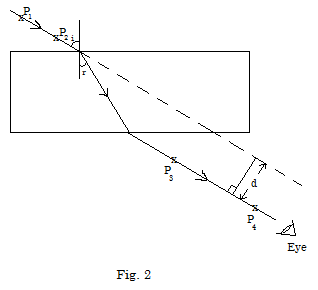
\includegraphics[width=10cm]{./img/2004-2-alt.png}
\end{center}

\begin{enumerate}
\item[(a)] Draw a line making an angle of incidence, $i$ of $30^\circ$. Erect two pins P$_1$ and P$_2$ on this line at a suitable distance apart. Replace the glass block and erect two more pins P$_3$ and P$_4$ at positions which appear to be in a straight line with the other two pins as seen through the glass block from the other side.\\[10pt]

Remove the glass block and draw the complete path of the ray (see Fig. 2). Measure the angle of refraction, $r$.
\item[(b)]
\begin{enumerate}
\item[(i)] Extend the direction of the incident ray as shown by the dotted line.
\item[(ii)] Measure the perpendicular distance `$d$' between extended incident ray and the emergent ray.
\end{enumerate}
\item[(c)] Repeat the procedure in (a) and (b) above for angles of incidence of $30^\circ$, $40^\circ$, $50^\circ$, $60^\circ$ and $70^\circ$. (In each case make your drawings on a fresh part of the drawing paper).
\item[(d)] Tabulate your results as shown in Table 1 below.
\begin{center}
\begin{tabular}{|p{0.15\textwidth}|p{0.15\textwidth}|p{0.15\textwidth}|p{0.15\textwidth}|p{0.15\textwidth}|} \hline
\multicolumn{1}{|c|}{$i$ (deg)} & \multicolumn{1}{c|}{$r$ (deg)} & \multicolumn{1}{c|}{$d$ (cm)} & \multicolumn{1}{c|}{$d\cos{r}$} & \multicolumn{1}{c|}{$\sin{(i-r)}$} \\ \hline
\multicolumn{1}{|c|}{30}&&&& \\
\multicolumn{1}{|c|}{40}&&&& \\
\multicolumn{1}{|c|}{50}&&&& \\
\multicolumn{1}{|c|}{60}&&&& \\
\multicolumn{1}{|c|}{70}&&&& \\ \hline
\end{tabular}\\[10pt]
\end{center}
\begin{enumerate}
\item[(i)] Plot a graph of $d\cos{r}$ against $\sin{(i-r)}$.
\item[(ii)] Find the gradient of the graph.
\item[(iii)] Measure the width of the glass block.
\item[(iv)] How is the gradient of the graph in 2 (a)(ii) and the width of the glass block in 2 (a)(iii) related?\\[5pt]
\end{enumerate}
\item[] NB: \quad Hand in your diagrams (drawings) together with your answer booklet. 
\item[] \flushright \textbf{(25 marks)}

\end{enumerate}

\item[3.] Determine the resistivity $\rho$ of the wire labelled W and the internal resistance of the battery provided.\\

Proceed as follows:

\begin{center}
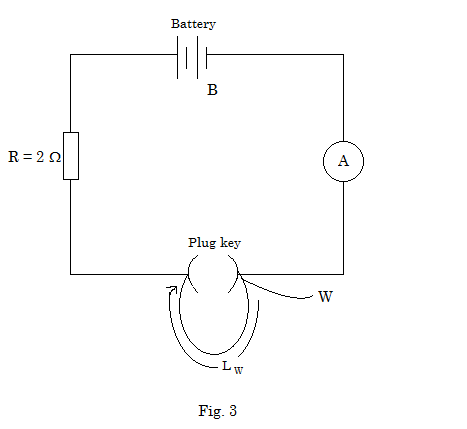
\includegraphics[width=10cm]{./img/2004-3-alt.png}
\end{center}

Connect the circuit as shown in fig. 3 above. With the plug key open adjust the length of wire W to a value of 20 cm. Note the ammeter reading.\\[10pt]

\noindent NB: The plug key should remain open throughout the experiment.

\begin{enumerate}
\item[(a)] Repeat the procedure above for $L_W$ = 40 cm, 60 cm, 80 cm and 100 cm each time recording the ammeter reading.
\item[(b)] Tabulate your results as shown in Table 2 below.

\begin{tabular}{|p{2.5cm}|c|c|} \hline
Length $L_W$ of wire (cm)& Current $I$ (A)& $\cfrac{1}{I} \left(\text{A}^{-1}\right)$ \\ \hline
&& \\
&& \\
&& \\
&& \\ \hline
\end{tabular}\\[10pt]

\item[(c)]
\begin{enumerate}
\item[(i)] Plot a graph of $\cfrac{1}{I}$ (vertical) against $L_W$ (horizontal).
\item[(ii)] Determine the slope G.
\item[(iii)] Determine the intercept $Y$ on the vertical axis.
\end{enumerate}
\item[(d)] Measure and record the diameter at four different places on the wire. Hence find the mean value of diameter $d$.
\item[(e)] Given that $G = \cfrac{4\rho}{\pi d^2E}$ and $Y = \cfrac{R + r}{E}$\\[10pt]
Where $E$ is the emf of the battery, and $R = 2 \Omega$, Find the
\begin{enumerate}
\item[(i)] Resistivity $\rho$ of the wire.
\item[(ii)]	Internal resistance $r$ of the battery. \hfill \textbf{(25 marks)}
\end{enumerate}
\end{enumerate}

\end{enumerate}
%\pagebreak
%\setcounter{secnumdepth}{2}